\documentclass[12pt]{article}
\usepackage[utf8]{inputenc}
\usepackage{fullpage}
\usepackage{graphicx}
\usepackage{enumitem}
\usepackage{hanging}
\usepackage{lipsum}
\usepackage{svg}
\usepackage{amsmath}
\usepackage{xcolor}
\usepackage{soul}
\usepackage{color}
\usepackage[usenames,dvipsnames]{xcolor}
\usepackage{lastpage} % Required to determine the last page number for the footer
\usepackage{graphicx} % Required to insert images
\setlength\parindent{0pt} % Removes all indentation from paragraphs
\usepackage[most]{tcolorbox} % Required for boxes that split across pages
\usepackage{booktabs} % Required for better horizontal rules in tables
\usepackage{listings} % Required for insertion of code
\usepackage{etoolbox} % Required for if statements
\usepackage{geometry} % Required for adjusting page dimensions and margins
\usepackage{wrapfig}
\usepackage{algorithm}
\usepackage{algorithmic}
\usepackage{hyperref}

\newcommand{\hlc}[2][yellow]{ {\sethlcolor{#1} \hl{#2}} }

\geometry{
	paper=a4paper, % Change to letterpaper for US letter
	top=3cm, % Top margin
	bottom=3cm, % Bottom margin
	left=2.5cm, % Left margin
	right=2.5cm, % Right margin
	headheight=14pt, % Header height
	footskip=1.4cm, % Space from the bottom margin to the baseline of the footer
	headsep=1.2cm, % Space from the top margin to the baseline of the header
	%showframe, % Uncomment to show how the type block is set on the page
}
\pagestyle{fancy} % Enable custom headers and footers



\title{ILP CW2}
\author{Yannik Nelson}

\begin{document}

\maketitle

\tableofcontents \newpage
\section{Introduction}
The project detailed in the coursework is to program an autonomous drone to collect readings from air quality sensors distributed around an urban geographical area as part of a research project to analyse urban air quality.\newline
This software is to be created with the intention of passing it on to a team who will maintain and develop it further.

\section{Software Architecture}
As mentioned in the introduction, this software is intended to be passed on to another team and further developed, as such it is important the the structure of the software is simple, and easy to make substantial changes to. For this reason I have decided have a strong focus on dependency inversion in the architecture of this software. The structure of the system was designed to minimise coupling and maximise cohesion for this reason too.
\subsection{Dependency Inversion}
Dependency Inversion is a principal intended to stress the decoupling of software modules. The principal states:
\begin{itemize}
    \item High-level modules should not depend on low-level modules. Both should depend on abstractions (e.g. interfaces).
    \item Abstractions should not depend on details. Details (concrete implementations) should depend on abstractions.
\end{itemize}
In order to achieve this I will be employing interface 'wrappers' around major components of the software to allow these modules to be more easily re-developed and replaced in the future.

\subsection{Class Structure and Motivations}
\begin{wrapfigure}[10]{l}{0.5\textwidth}
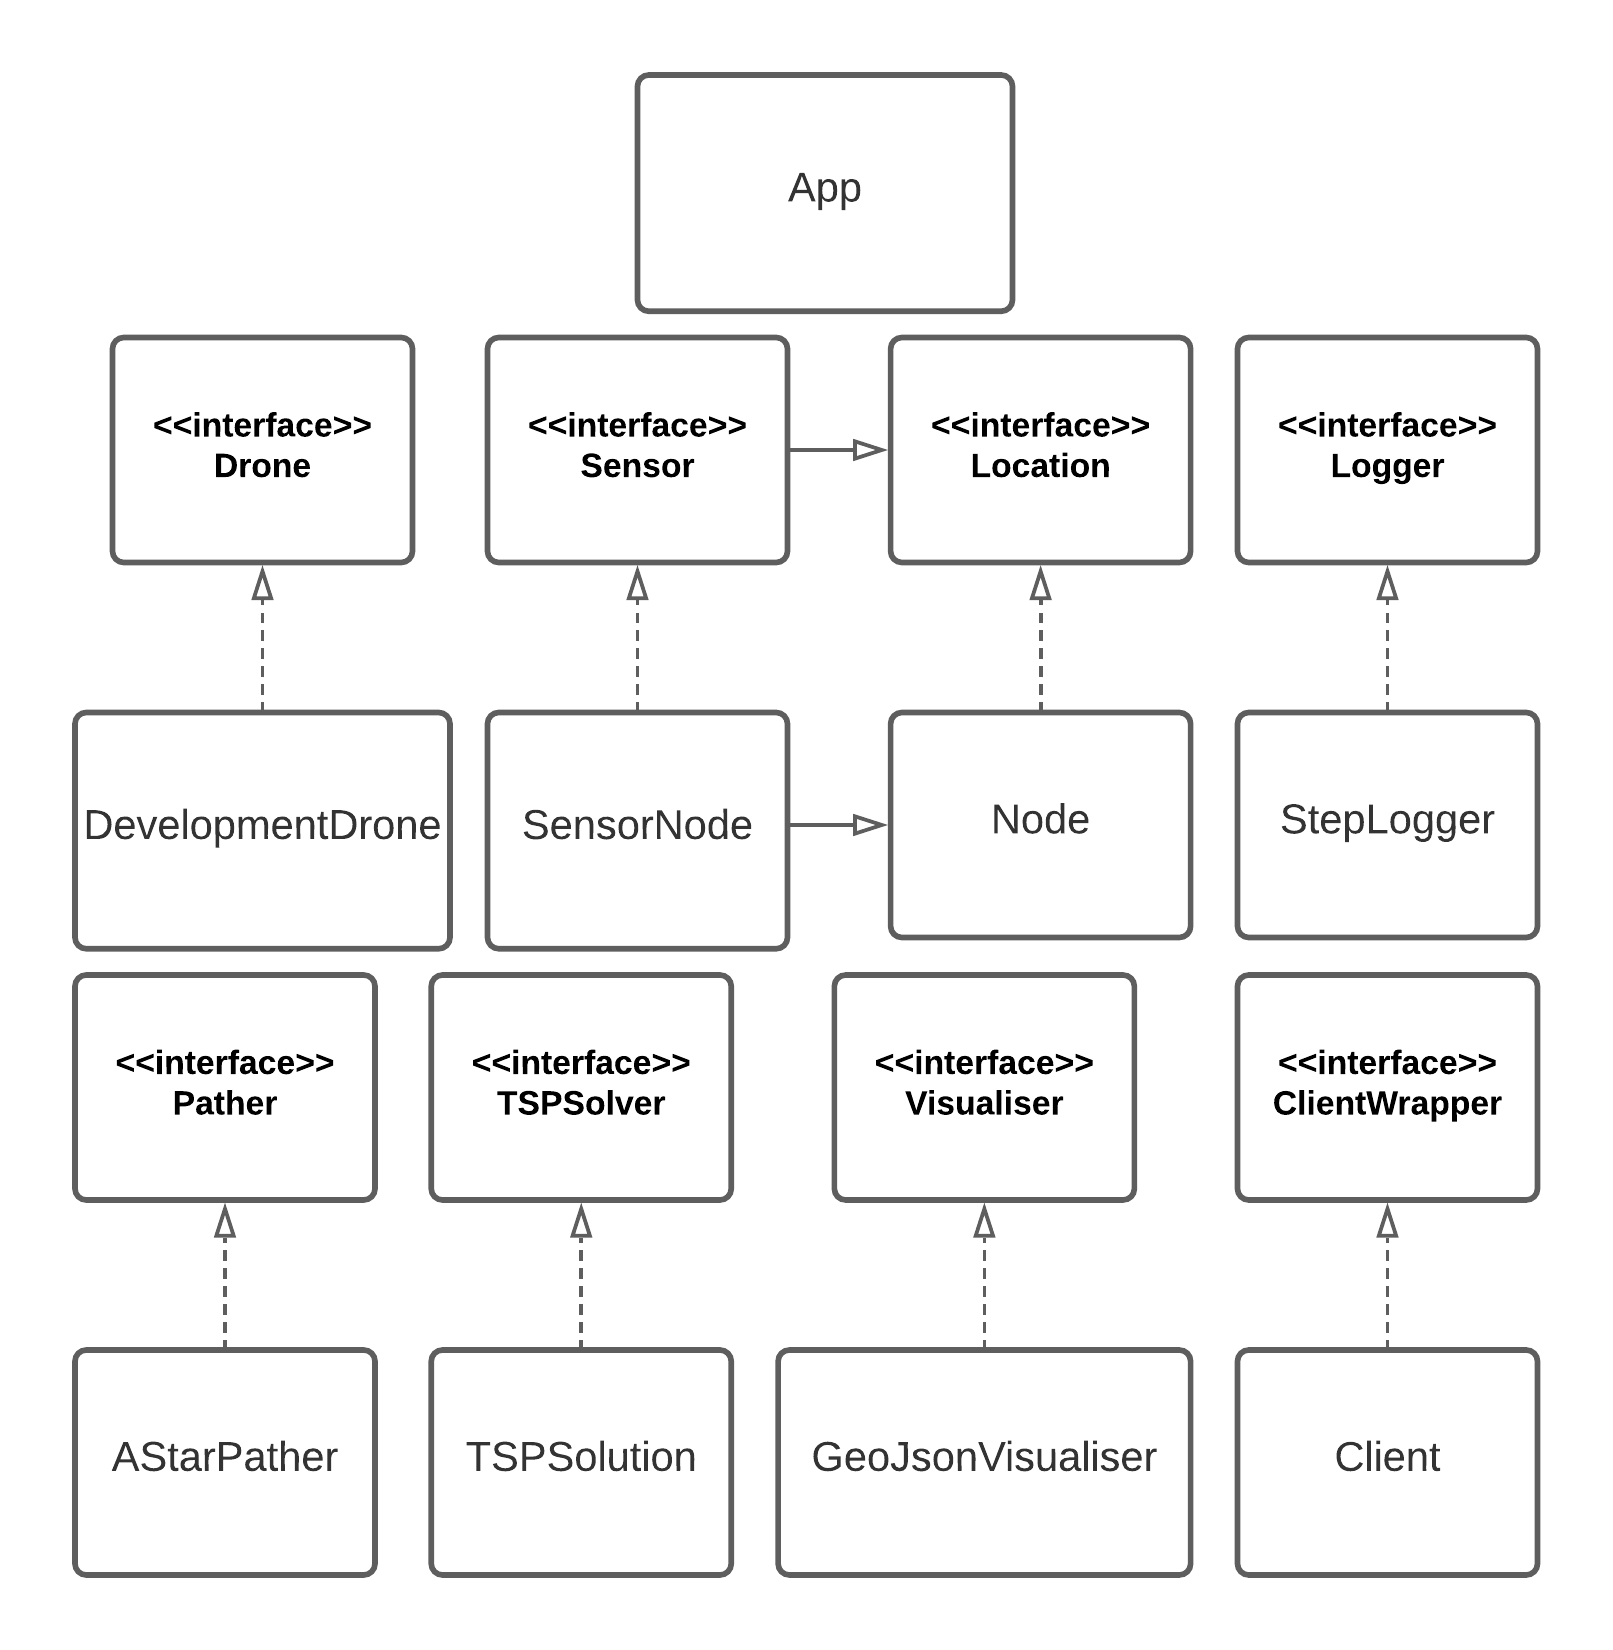
\includegraphics[width=0.4\textwidth]{ILP Basic Class Diagram.png}
\end{wrapfigure}
Here you can see the basic class structure I'll be using. 
\subsubsection{The App Class}
The App class is present to simulate the drone receiving requests using the other classes to fulfill those requirests.
\subsubsection{The Development Drone Class and Drone Interface}
The Drone Interface is present in order to allow for multiple drone implementations and the Development Drone class implements this interface for the drone detailed in the brief.
\subsubsection{The Location Interface}I have a Location interface in order to abstract away the dependency on the mapbox library in the case the researchers decide to use another library in the future.
\subsubsection{The Sensor Interface}
The Sensor interface details the functions that will be required of any sensor representation. This mainly consists of getters and setters that supply required information about each sensor such as the reading and battery level. As can be seen from the diagram, the Sensor Interface extends the Location Interface, this is as we will want to be able to use Sensors as locations to reach.
\subsubsection{The Node and SensorNode Classes}
The Node and SensorNode classes implement the Location and Sensor interfaces respectively. As with the Sensor and Location interfaces, the SensorNode extends the Node class in order to maintain a consistent output for our locations.
\subsubsection{The Client Class and  ClientWrapper Interface}
In the brief we are told that we will be getting our data from a webserver, but this is likely not going to be the case in a practical implementation of this project. As such the ClientWrapper interface defines the methods the drone will use to get data from sensors etc.., the Client class implements these methods for a webserver.
\subsubsection{The AStarPather Class and Pather Interface}
For my solution I intend on using an AStar implementation to find paths from one Location to another but in the future the researchers may want to use a different, more efficient algorithm or implementation of AStar, as such I have created a Pather Interface that will be used for any class that implements the path finding for the drone.
\subsubsection{The TSPSolution Class and TSPSolver Interface}
The drone will not only have to get from one Sensor to another, it will have to decide in what order in which to visit the Sensors in order to minimise the number of steps it takes. This is the Travelling Salesman Problem (TSP) and as such the drone will need to be able to solve the TSP for 34 destinations (as the drone will have to visit 33 Sensors and return to its starting position each day). There are many implementations of solutions for TSP and the researchers will likely have a preference as to which they would like to use, as such a TSPSolver interface was created in order to standardise and simplify the replacement of TSP implementations.
\subsubsection{The GeoJsonVisualiser Class and Visualiser Interface}
The brief requires the system to output a GeoJson file contining Points for all of the Sensors and a Line for the path the drone took flying to all of them. This requirement is fulfilled by the GeoJsonVisiualiser class but the visualisation requirements may change in the future or better visualisation libraries may come into existence and as such this functionality is abstracted by the Visualiser Interface.
\subsubsection{The StepLogger Class and Logger Interface}
The brief requires the system to output a text file detailing each step the drone took in a specified format, this functionality is handled by the StepLogger Class by the format may change and as such this functionality is abstracted by the Logger interface for easier replacement.
\subsection{Basic Sequence Diagram}
\begin{center}
    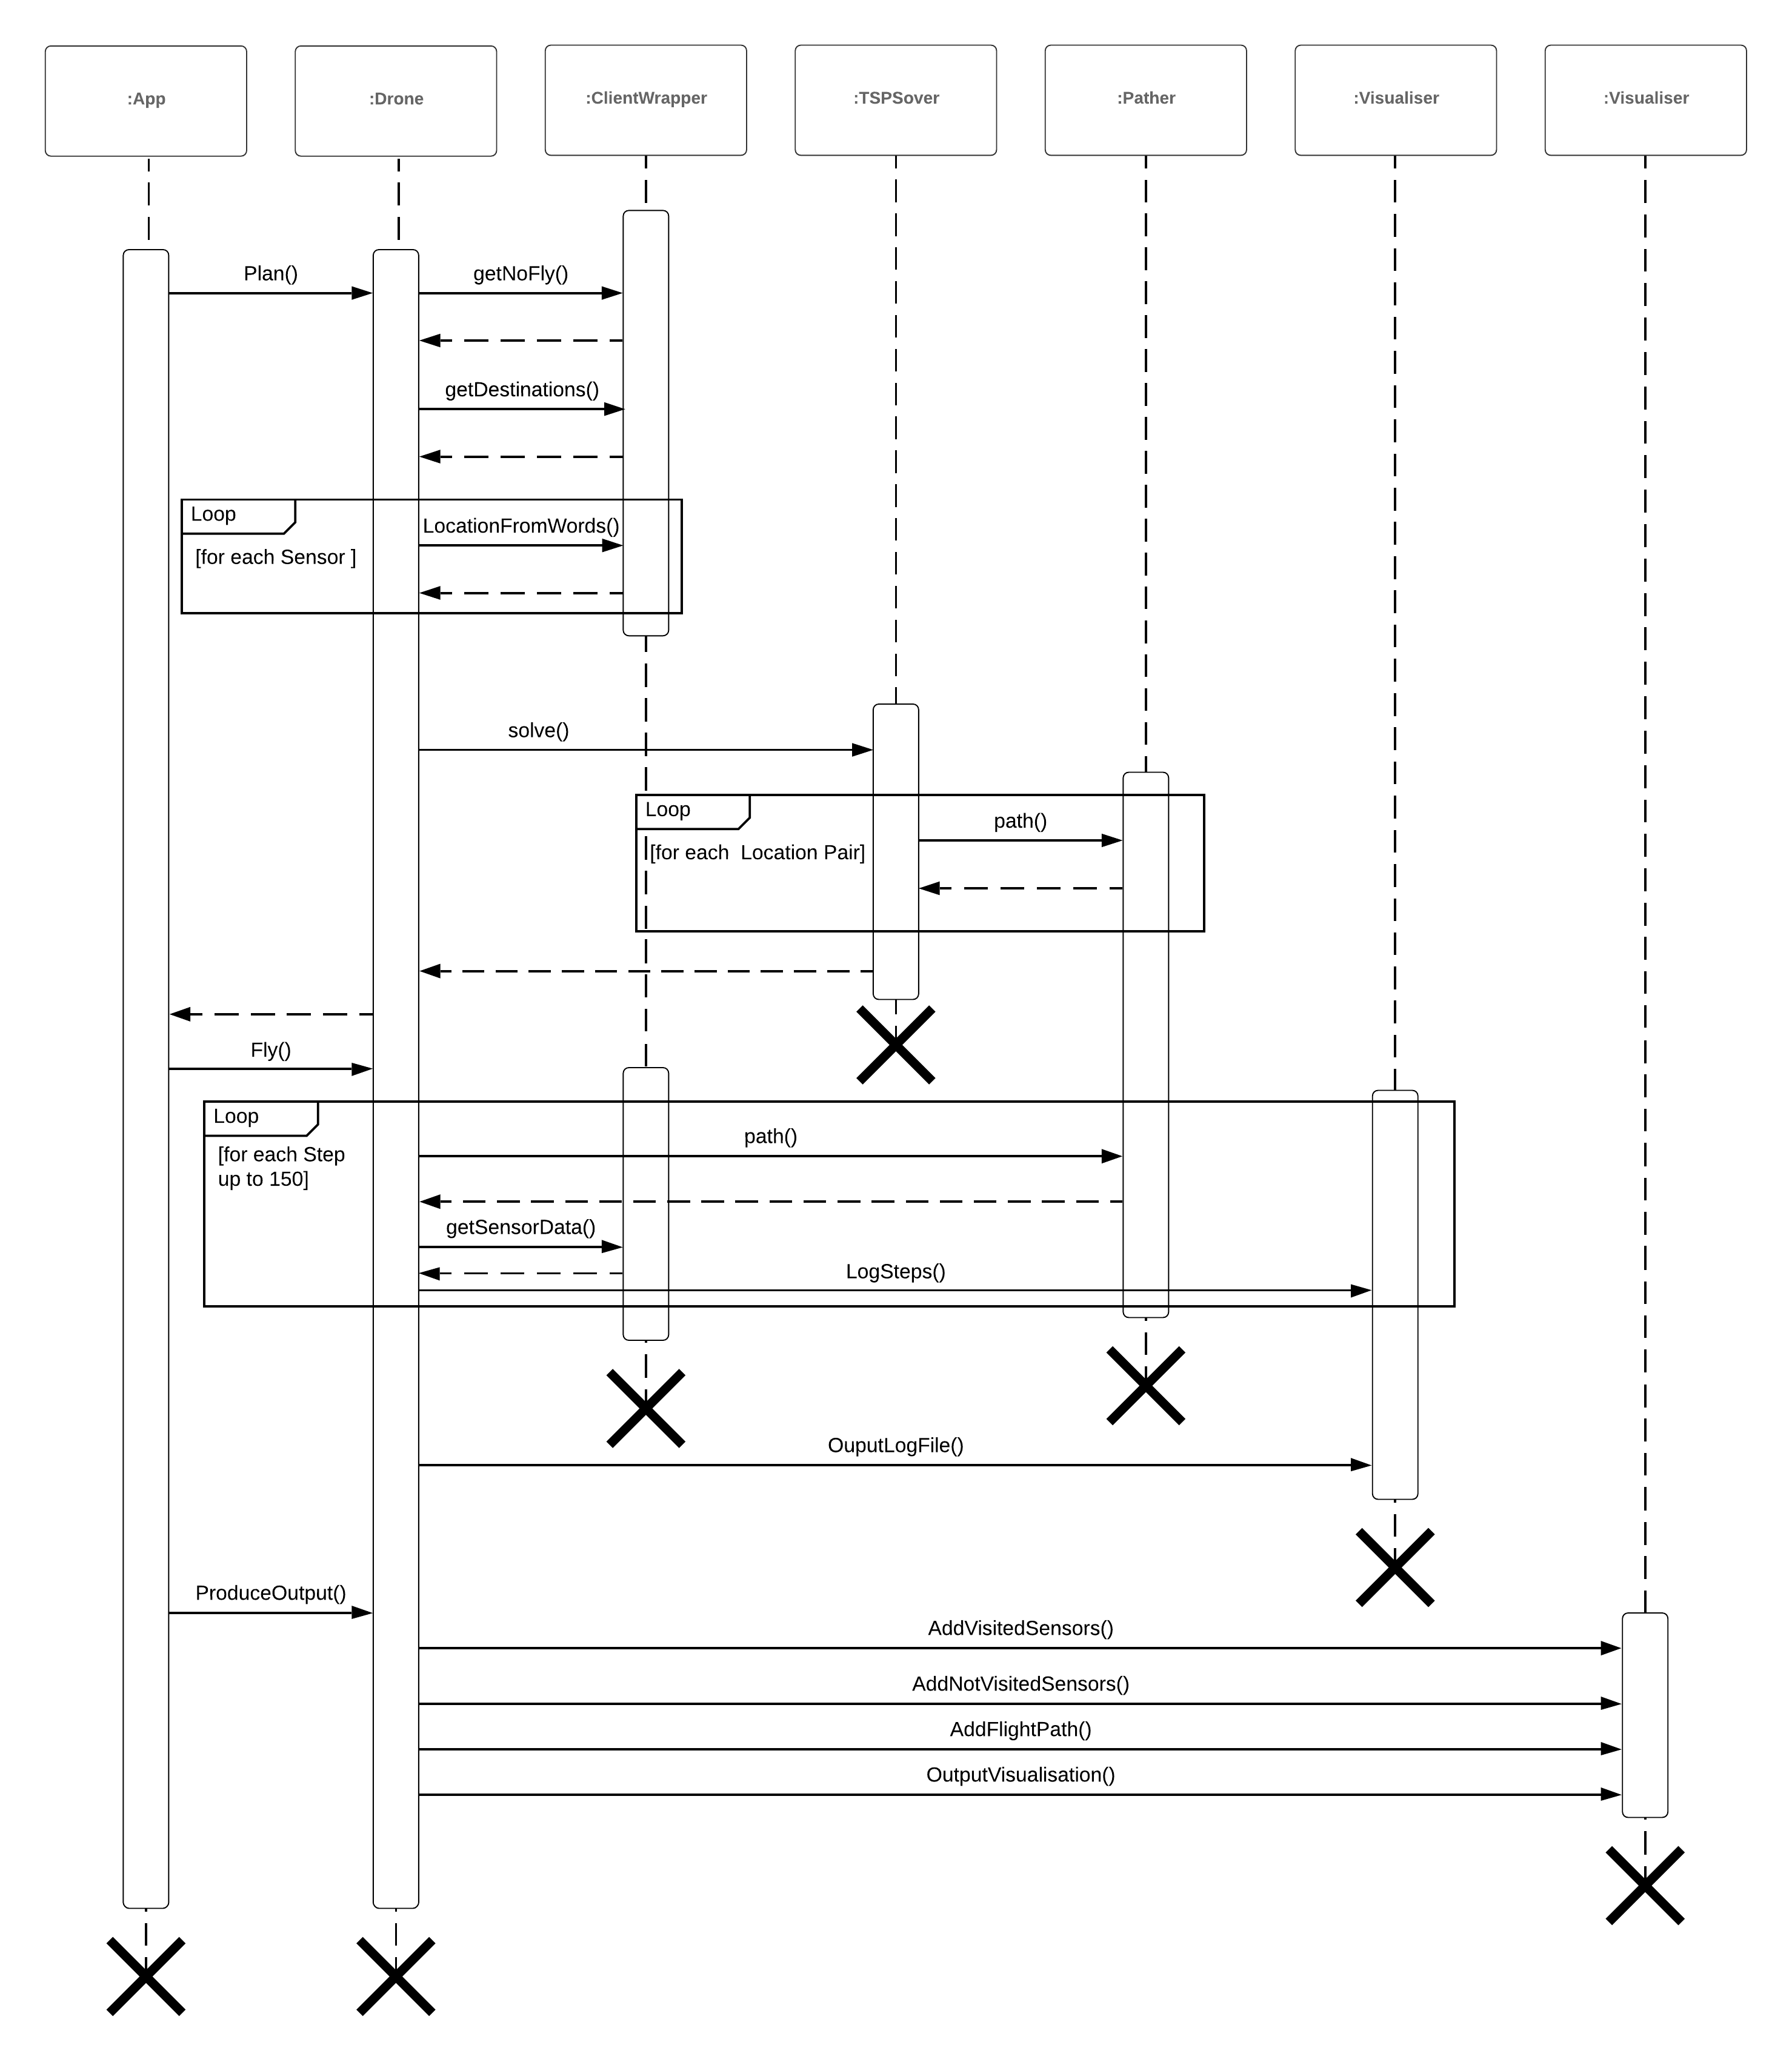
\includegraphics[width=0.83\textwidth]{Drone Sequence Diagram.png}
\end{center}
\newpage

The above sequence Diagram details the expected interaction between objects in the planning an flying phases of the system. To reduce clutter I have excluded the calls to get location data from Location and Sensor instances (in my implementation Node and SensorNode instances). I have also excluded how the TSPSolver and Pather produce thier results internally as it is not integral to the architecture of this software as well as how the Logger is used to ensure the number of steps output stays below or equal to 150.
\section{Class Documentation}
\begin{wrapfigure}[28],
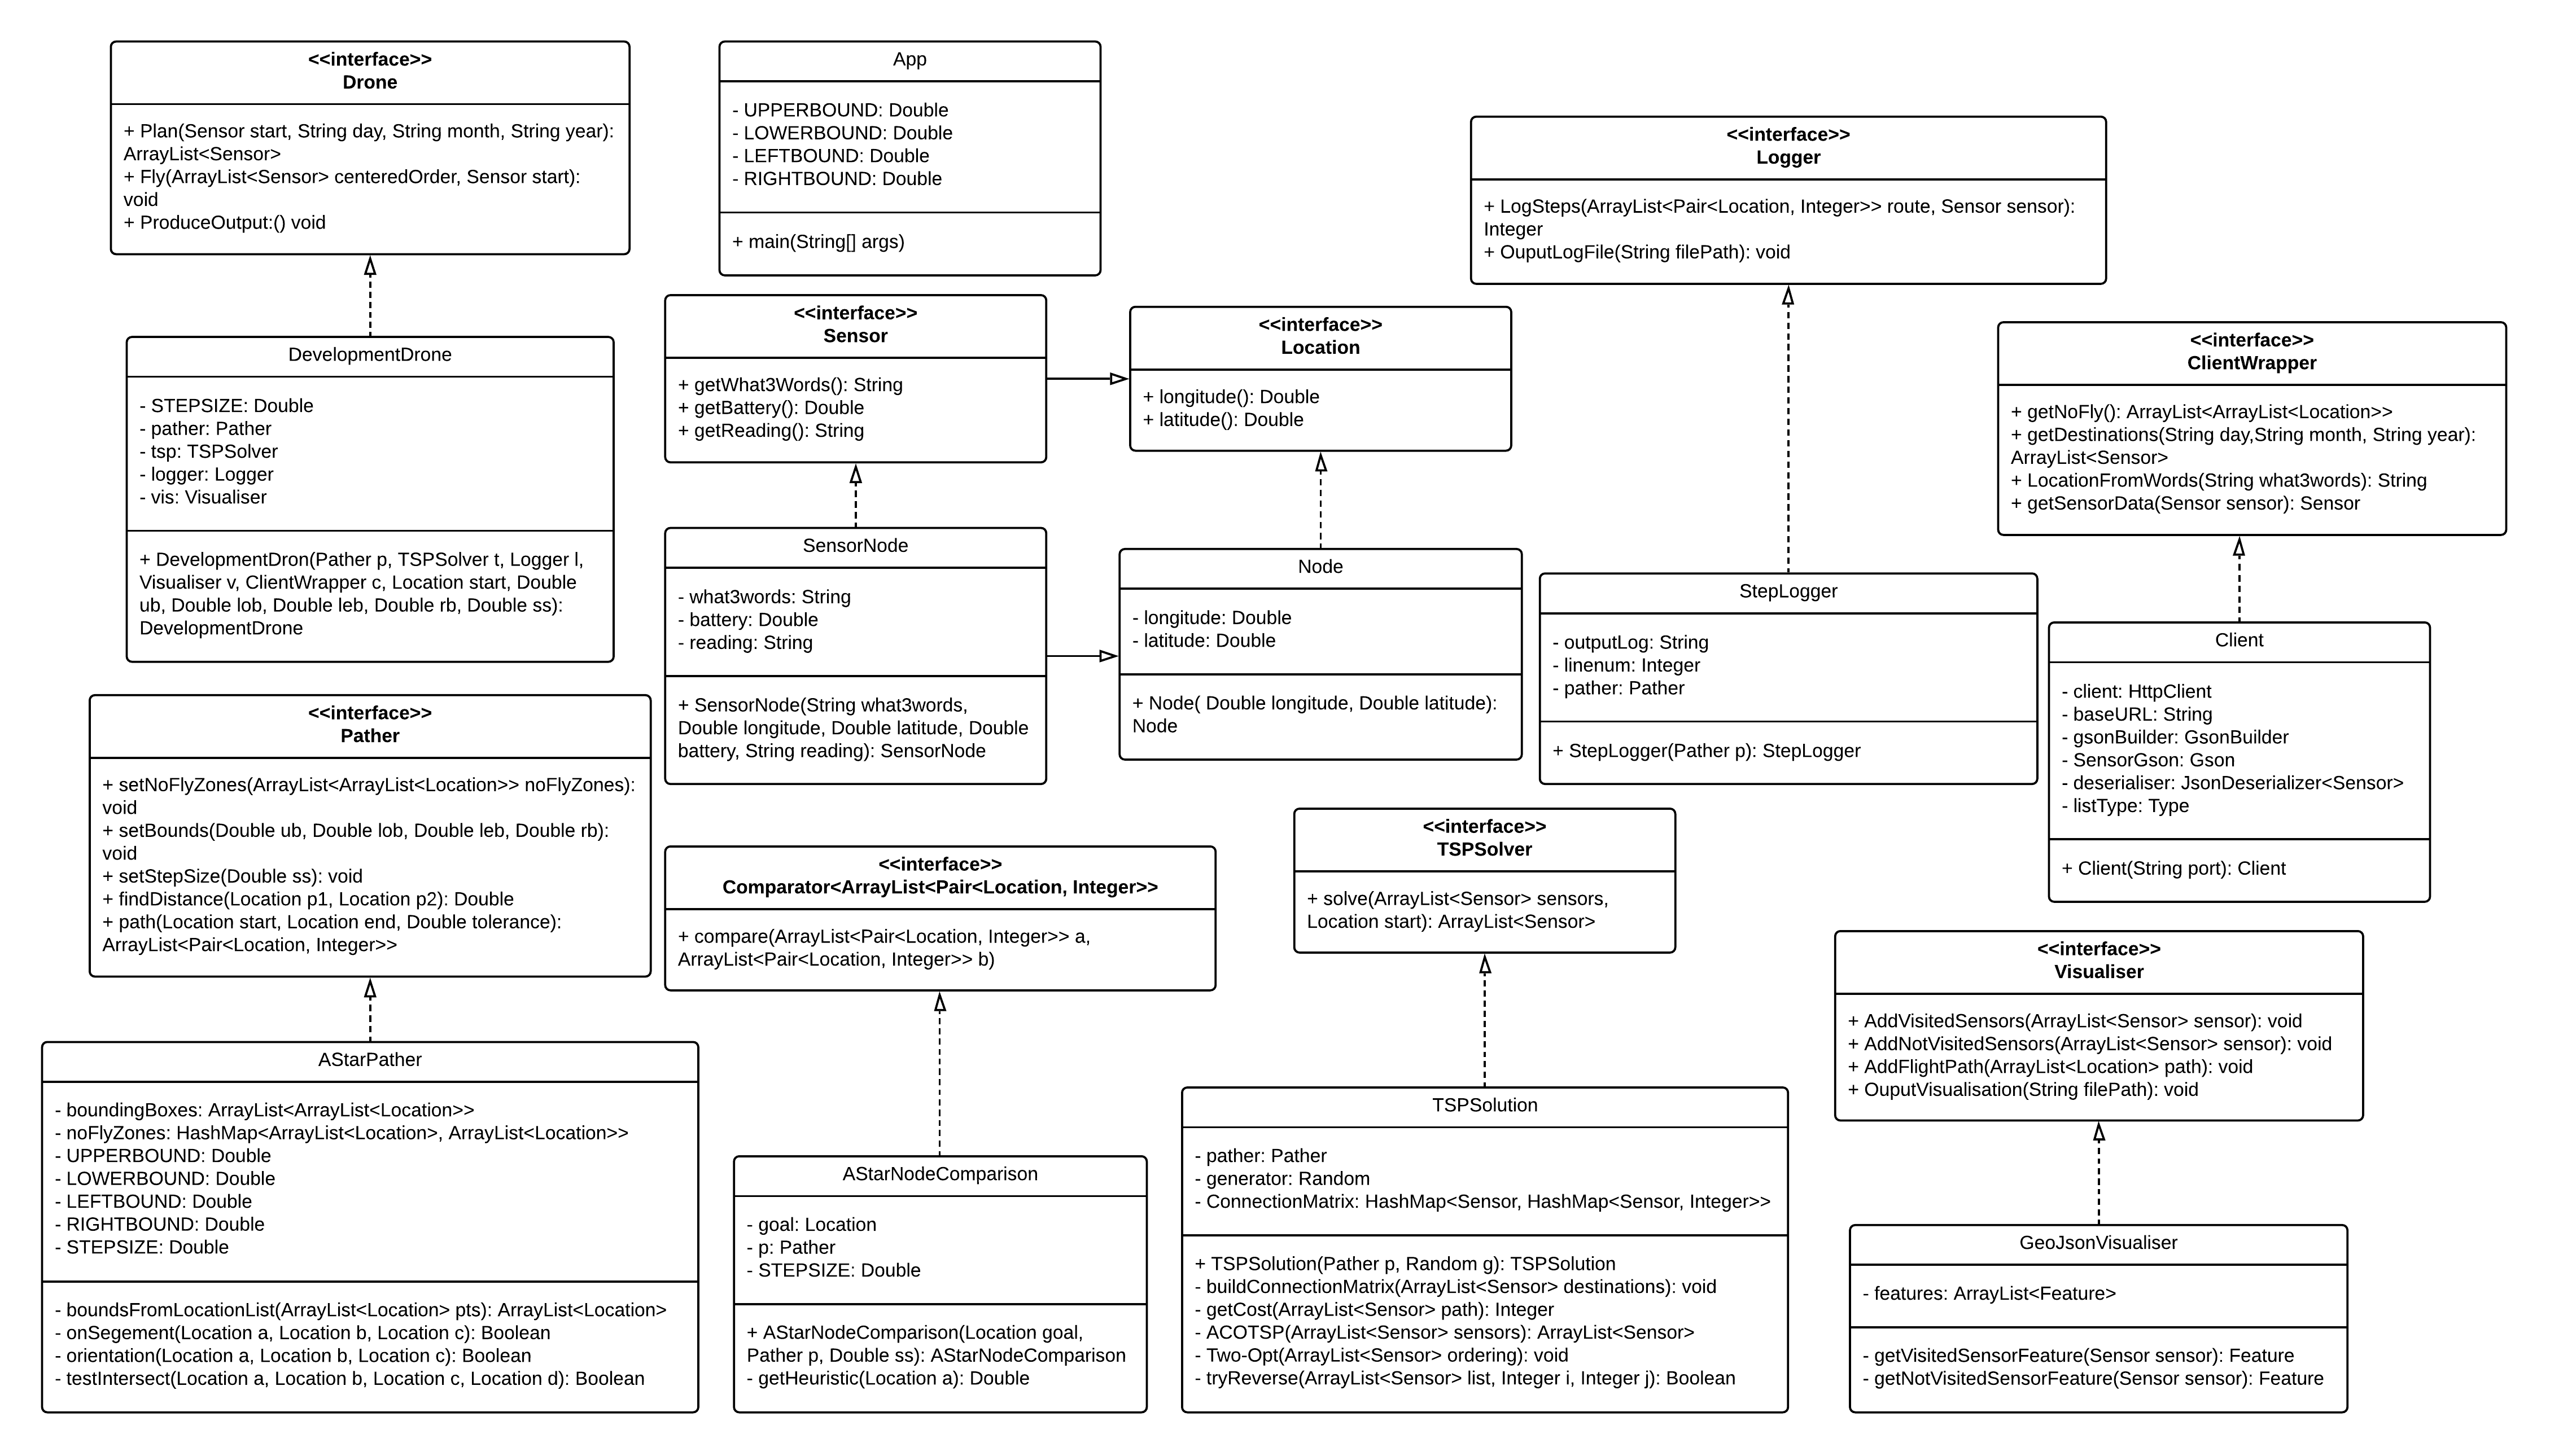
\includegraphics[width=1.15\textwidth, angle=90]{Detailed Class Diagrams.png}
\end{wrapfigure}
The class diagram to the left gives a more detailed view of the classes used in my implementation of this project. \newline
\newline
In the diagram I have detailed the required functions of each interface and the attributes and extra functions each of my classes use.\newline
\newline
For my implementation I will require an implementation of the Comparator interface that can order potential paths based on their heuristic value, this is called AStarNodeComparison. I excluded this from the basic class diagram as it's specific to my implementation and not required for the general case of this problem.\newline
\newline
In the following sections I shall detail the functions of each interfaces' and class's functions.
\newpage
\subsection{Interfaces}
\subsubsection{Location}
This interface defines the functionality required by any representation of a location on the map. The functions are longitude() and latitude() and they return the longitude and latitude values respectively at Double precision.
\subsubsection{Sensor}
This interface extends the Location interface detailing the functionality required by any representation of a Sensor. The functions added to the Location functionality are: getWhat3Words() which returns the what3words coordinate of the Sensor as a String; getBattery() which returns the battery level of the Sensor with Double precision; and getReading() which returns the reading from the sensor as a String, String is used as this value received from the actual sensor can be "null" or "NaN".
\subsubsection{ClientWrapper}
The ClientWrapper Interface defines the minimum functionality of a client module of the drone, this is the module that communicates with 'the outside world' and gets required data. This functionality includes: getNoFly() which gets and returns a list of the areas the drone is not allowed to fly over*; getDestinations() which gets the list of sensors to be visited on the passed in date converting the recieved data into the internal Sensor representation; LocationFromWords() which will get the location data for the passed in what3words string and return the internal location representation for that location; and getSensorData() which takes in a Sensor the drone believes it's in range of and return a Sensor object containing the readings and battery level. \newline
\newline
*Each no-fly-zone is represented as a list of Locations corresponding the vertexes of the zone's perimeter, this list is ordered so that each location-vertex is preceded and followed by the previous and next in the perimeter respectively.
\subsubsection{Pather}
This defines the expected functionality from any pathing modules the drone uses. setNoFLyZones() takes in and saves the areas to be avoided (in the form described above). setBounds() takes in and saves max and min values (with Double Precision) for the allowed longitude and latitude defining the bounds of the area in which the drone is allowed to fly. setStepSize() takes in and saves the length each step the drone takes must be (with Double precision). findDistance() takes in two Location and returns the distance between them (with Double precision). Finally path() which takes in a starting Location, an end Location and a tolerance (Double precision) and attempts to find a path starting at the starting Location and ending within the tolerance of the end Location while remaining within the bounds and avoiding the no-fly-zones.
\subsubsection{TSPSolver}
As mentioned before, the drone will require the ability to solve the Travelling Salesman Problem in order to minimise the steps it requires to travel to every sensor. The TSPSolver interface defines the function format that will be used to interact with any TSP Solution: solve() takes in a list of sensors to be visited and a star Location and returns the of Sensors in the order they should be visited.
\subsubsection{Logger}
The Drone is required to Log and save the details of each step it takes. This interface details the required functionality of any module that provides this logging. LogSteps() takes in a list of Locations paired with Integers which represent Locations the drone visited and the angle the drone flew at to reach that Location and a Sensor the Drone attempted to read at the end of that series of steps, this list is expected to be the path from one sensor to the next, not the complete path. OutputLogFile() which takes a path (or filename) and saves the log file to that location(/file).
\subsubsection{Visualiser}
The Drone is also required to output a visualisation of its activities including all of the sensors it visited, all the sensors it didn't visit and the path it flew. This Interface details the required functionality of any module that performs this visualisation: AddVisitedSensors() takes in a list of Sensors that the drone has visited and adds them to the visualisation; AddNotVisitedSensors() takes in a list of Sensors that the drone failed to visit and adds them to the visualisation; AddFlightPath() takes in a list of Locations that the drone visited, in the order it visited it and adds it to the visualisation; and finally OutputVisualisation() which takes a path (or filename) and saves the visualisation to that location(/file).
\subsubsection{Drone}
Finally there's the Drone interface which dictates the activities the drone itself will perform: Plan() the functionality of planning the route and returns said route; Fly() flying the route previously planned returning nothing; and ProduceOutput() which will return nothing but save the log and visualisation for the flight.
\subsection{Classes}
\subsubsection{Node}
This is my implementation of the Location interface, Initially this stored a MapBox Point and the functions simply acted as wrappers, but this added a lot of overhead and slowed the process down significantly, as such this class now simply stores the longitude and latitude values and outputs them when requested.
\subsubsection{SensorNode}
This is the implementation of the Sensor interface, it extends the Node class and performs similar operatiosn for the Sensor data.
\subsubsection{Client}
The Brief of the project stated that all the data would be stored on a web-server, as such the client module that the drone needs to use in development is an HttpClient, this class holds that client and performs the necessary operations to get the required data from the server. At instantiation, the Client expects the port number of the webserver.
\subsubsection{AStarPather}
For my pathing solution I decided I would be using the AStar algorithm. I also implemented some optimisations for object avoidance which will be detailed in the Algorithm Section of this Report
\subsubsection{TSPSolution}
My TSPSolver implementation TSPSoltuion is a combination of the Ant Colony Optimisation and 2-Opt Heuristic. Both of these implementation require knowledge of each possible connection between destinations and the length of those connections. As such two helper functions have been created that both of these algorithms use, buildConnectionMatrix() which uses the Pather to estimate the number of steps required to get from one Sensor to another (also including the starting Location in the form of a Sensor) taking in a list of Sensors and saving the resulting matrix returning nothing; getCost() which takes in a potential ordering of Sensors and evaluates the expected step cost. \newline
These functions are used by ACOTSP() which implements the Ant Colony Optimisation for the passed in list of destinations (sensors) assuming the connection matrix contains at least those sensors and returns the optimum order it found; and Two\_Opt() which implements the 2-opt heuristic algorithm using the tryReverse() fuction to reverse sub-sections of the list for readability.
\subsubsection{StepLogger}
The StepLogger class implements the Logger interface. For my implementation, before adding a sensor read to the log, I ensure the drone is within range of said sensor, this requries the get distance function from the Pather implementation and as such the StepLogger requires a Pather instance in its constructor.
\subsubsection{GeoJsonVisualiser}
The GeoJsonVisuliser is the implementation of the Visualiser interface for outputting a GeoJson visualisation. It does this using the MapBox library. Two helper functions are used getVisitedSensorFeature() and getNotVisitedSensorFeature() which both take in a Sensor object and return a MapBox Feature consisting of a Point with the appropriate properties for if the sensor had been visited or not.
\subsubsection{DevelopmentDrone}
The DevelopmentDrone is the implementation of the Drone interface used for this development. It directly implements the interface with no extra functions needed, though it's constructor takes in a Pather object, a TSPSolver object, a Logger object, a Visualiser object, a ClientWrapper object and details about its start Location and permitted fly area. The Constructor was made this way to facilitate easy of testing with mock objects and to make swapping out interface implementations easy as you need only provide a different object to the drone.
\subsubsection{App}
This is the main class of the project. The main of this class is used to instantiate the instance of all the required objects (bar the Locations and Sensors) and calling the Drone's Plan, Fly and ProduceOutput() functions.
\section{Drone Control Algorithm}
\subsection{AStar Pathing Algorithm}
For pathing and object avoidance I decided to use the AStar algorithm as it has a simple implementation and should give the optimal result in a short time. My AStar implementation works as such
\begin{algorithm}
 \caption{path(Location Start, Location End, Double tollerance):}
 \begin{algorithmic}[1]
  \STATE create an empty list of branches to search, call this list branches
  \STATE create the first branch consisting of the Start and add it to the list
  \STATE create a list of visited Locations containing the start Location
  \WHILE{True}
  \STATE current = the first branch in branches
  \IF{current ends within the tollerance of End}
  \RETURN current
  \ENDIF
  \STATE available = list of all next possible Locations from current
  \STATE remove current from branches
  \FOR{Each Location l in available}
  \IF{l is not in visited}
  \STATE create a copy of current, place l as the end, add this branch to branches
  \ENDIF
  \ENDFOR
  \STATE sort branches by the heuristic value of each branch
  \STATE add the last Location from current in visited
  \ENDWHILE
 \end{algorithmic}
\end{algorithm}
Each branch consists of a list of pair of Locations and Integers, Location is a Location visited by the drone, the Integer is the angle the drone flew at to reach that Location, conceptually we shall ignore the Integer for AStar.

This algorithm in itself does not have any object avoidance in it. I produced the object avoidance in the function that gets next possible locations:
\begin{algorithm}
\caption{Reachable(Location Current, List$\langle Location \rangle$ Visited):}
\begin{algorithmic}[1]
 \STATE nextPoints = and Empty list of pairs of Locations and Integers
 \STATE OuterLoop:
 \FOR{i from 0 to 355 increasing by 5 (We run through every angle the drone can move at (every multiple of 5))}
    \STATE long = Longitude after from moving the stepsize from current Location at angle i
    \IF{long is out of bounds}
    \STATE continue OuterLoop
    \ENDIF
    \STATE lat = Latitude after from moving the stepsize from current Location at angle i
    \IF{lat is out of bounds}
    \STATE continue OuterLoop
    \ENDIF
    \STATE newLoc = Location made from long and lat
    \FOR{Each Visited Node v}
    \IF{newLoc is within a step of v}
    \STATE continue OuterLoop
    \ENDIF
    \ENDFOR
    \FOR{Each no-fly-zone bounding box b}
    \IF {The line segment from the current Location to newLoc intersects the bounding box}
    \FOR{Each line segment l of the no-fly-zone perimeter}
    \IF{The line segment from the current Location to newLoc intersects l}
    \STATE continue OuterLoop
    \ENDIF
    \ENDFOR
    \ENDIF
    \ENDFOR
    \STATE Add the Pair of newLoc and i to next Points
 \ENDFOR
 \RETURN nextPoints
\end{algorithmic}
\end{algorithm}
\newline
This algorithm finds all the possible next Locations a drone could visit from a given Location, and removes any that are close to a Location already visited and any Locations that would require the drone to enter an area in which it is not allowed.\newline \newline
The code for checking the intersection of two line segments was taken from here:\newline
\url{https://www.geeksforgeeks.org/check-if-two-given-line-segments-intersect/}
\newpage

\subsection{Travelling Salesman}
\subsubsection{Connection Matrix Creation}
Both of my TSP algorithms require a look up table from one destination to another containing the expected cost to travel from the first the the second, here is the algorithm I used to create said table:
\begin{algorithm}
\caption{buildConnectionMatrix(List$\langle Sensor \rangle$ list):}
\begin{algorithmic}[1]
 \STATE connectionsMatrix = HashMap Indexed by Sensors holding a HashMap Indexed by Sensors holding Integers
 \FOR{Each Sensor to in list s}
 \STATE connectionsMatrix.put(s, new HashMap Indexed by Sensors holding Integers)
 \ENDFOR
 \FOR{Each Sensor in list s1}
 \FOR{Each Sensor in list s2}
 \IF{s1 == s2}
 \STATE connectionsMatrix.get(s1).put(s2, 0)
 \ELSE
 \STATE connectionsMatrix.get(s1).put(s2, pather.path(s1, s2, 0.0002).size())
 \ENDIF
 \ENDFOR
 \ENDFOR
\end{algorithmic}
\end{algorithm}
This function creates a mapping from a combination of two Sensors s1 and s2 to an Integer equal to the estimated number of step to reach s2 from s1 (+1 to allow for inconsistencies in tolerances and starting positions). \newline
To keep track of the progress of producing this matrix i have used the ProgressBar library: \url{https://tongfei.me/progressbar/}
\subsubsection{Path Evaluation}
Both of the algorithms also need to be able to measure the cost of a produced route:
\begin{algorithm}
\caption{getCost(List$\langle Sensor \rangle$ list):}
\begin{algorithmic}
 \STATE total = 0
 \FOR{Each index in list starting at the second element}
 \STATE total += connectionMatrix.get(list.get(index-1).get(list.get(index))
 \ENDFOR
 \STATE total += connectionMatrix.get(list.get(last index).get(list.get(0))
 \RETURN total
\end{algorithmic}
\end{algorithm}
This sums the lengths of every connection in the route (including the return to the starting Sensor).
\newpage
\subsubsection{Ant Colonly Optimisation TSP Solution}
The first part of my TSP solution is to run the Ant Colony Optimisation. This works by simulating a series of ants traversing the connections of the 'graph' and laying down pheromone as they go, with their decision guided by connection lengths and pheromone strengths:
\begin{algorithm}
\caption{ACOTSP(List$\langle Sensor \rangle$ list):}
\begin{algorithmic}[1]
 \STATE pheromone = copy of connectionMatrix with 1 at every Mapping
 \STATE ants = empty List of Lists of Sensors
 \STATE best = copy of list
 \State bestCost = getCost(best)
 \FOR{t from 0 to 99}
 \FOR{k from 0 to the size of list}
 \STATE possibleNext = copy of list
 \STATE ant = new empty List of Sensors
 \STATE pick a random Sensor from possibleNext and add it to ant and remove it from possibleNext
 \WHILE{possibleNext is not empty}
 \STATE pick a next Sensor from possibleNext with probability based off of the length of the connection to that sensor and the pheromone strength on that same connection (equation bellow).
 \STATE Add the chosen Sensor to ant and remove it from possibleNext
 \ENDWHILE
 \STATE Add ant to ants
 \ENDFOR
 \STATE Apply evaporation to the pheromone Matrix by multiplying every element in it by 1-evap
 \FOR{every ant in ants}
 \STATE currentCost = getCost(ant)
 \IF{currentCost $<$ bestCost}
 \STATE best = ant
 \STATE bestCost = currentCost
 \ENDIF
 \FOR{each connection the ant travlled down}
 \STATE update that connection's pheromone strength by adding $\frac{1}{currentCost}$
 \ENDFOR
 \ENDFOR
 \RETURN best
 \ENDFOR
\end{algorithmic}
\end{algorithm}

\[prob = \frac{p_{pn, c}^a + \frac{1}{d_{pn, c}}^b}{\sum_{next} p_{next, c}^a + \frac{1}{d_{next, c}}^b}\]
The probability of moving to Sensor pn from Sensor c is the strength of the pheromone on that connection + 1\textbackslash the length of that connection (raised to the power of b), all divided by the sum of that calculation for every possible next Sensor. This equation allows the ants to take into account both the length of a connection and the pheromone on it for influencing the paths they take, raising the pheromone and inverse of the distance to powers a and b respectively allow us to weight how important each factor should be when deciding where to go next.
\subsubsection{2-Opt Heuristic TSP Solution}
The 2-Opt Heuristic algorithm works by reversing every subsection of a route and seeing if that action improved the cost of the route. If the cost improved by reversing any subsection, then this process is run again until no improvement is found by reversing a subsection of the route. Her is the pseudocode for my implementation:
\begin{algorithm}
\caption{Two\_Opt(List$\langle Sensor \rangle$ list)}
\begin{algorithmic}
 \STATE better = True
 \WHILE{better}
 \STATE better = False
 \FOR{Integer j from 1 to the size of the list}
 \FOR{Integer i from 0 to j}
 \STATE better = tryReverse(list, i, j)
 \ENDFOR
 \ENDFOR
 \ENDWHILE
\end{algorithmic}
\end{algorithm}
\begin{algorithm}
\caption{TryReverse(List$\langle Sensor \rangle$ list, Integer i, Integer j)}
\begin{algorithmic}
 \STATE Intial = getCost(list)
 \WHILE{better}
 \STATE better = False
 \STATE reverse sublist of list from i to j in place
 \IF{getCost(list) $Initial$ Intial}
 \RETURN True
 \ENDIF
 \STATE reverse sublist of list from i to j in place again (to undo the change)
 \RETURN False
 \ENDWHILE
\end{algorithmic}
\end{algorithm}
The Algorithm for the Ant Colony Optimisation and the idea to run the Two-Opt heuristic on the rest was from:
\url{https://www.sciencedirect.com/science/article/pii/S1002007108002736#fd1}
\newpage
\section{Examples}
Bellow are two examples of paths produced by this system:
\begin{center}
    \begin{tabular}{c c}
    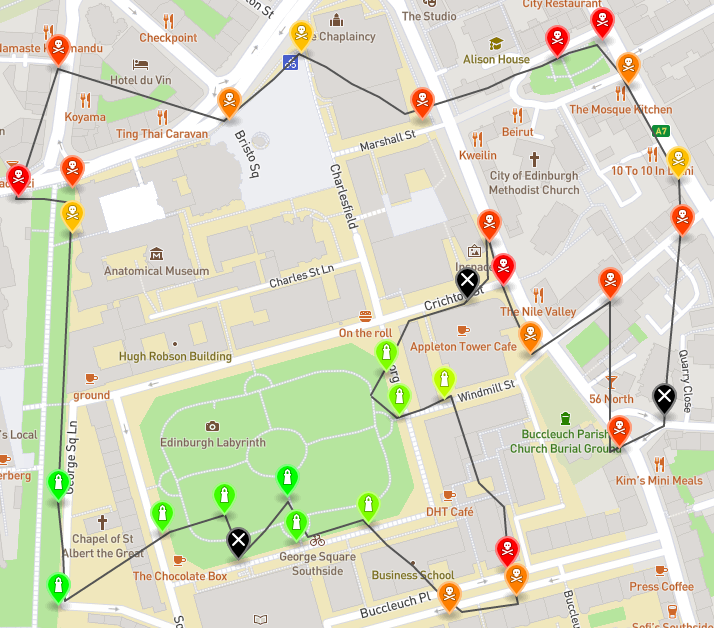
\includegraphics[width=0.3\textwidth]{example15-01-2021.png} &
    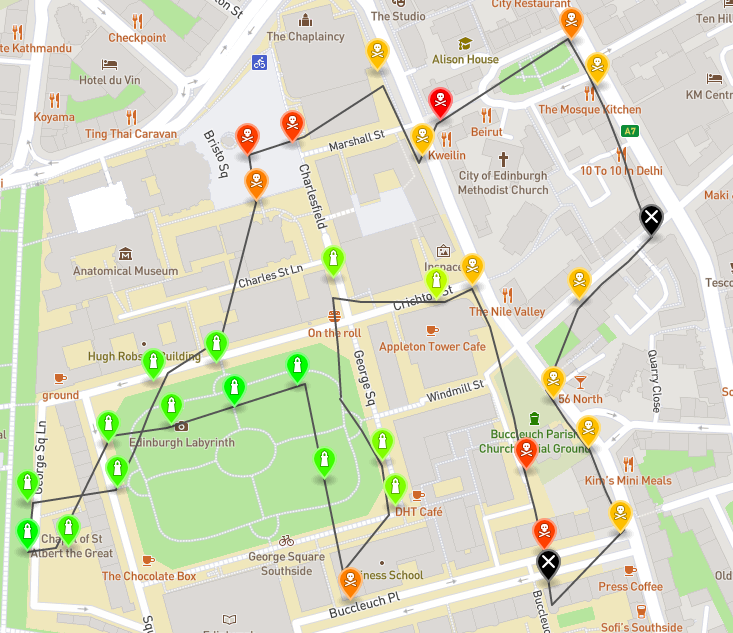
\includegraphics[width=0.3\textwidth]{example15-06-2021.png} \\
    \caption{Path From 15/01/2021} &
    \caption{Path From 15/06/2021}
\end{tabular}
\end{center}
Both of these examples used the same random seed and starting position:
\begin{tabular}{c c c}
    seed & latitude & longitude \\
    5678 & 55.944 & -3.1878
\end{tabular}\newline
The first example (15/01/2021) took 15 seconds and 85 steps to complete. The second example (15/06/2021) took 29 seconds and 76 steps to complete.
\section{Additional Dependencies}
I shall now list all of the sources mentioned and dependencies used in this project:
\subsection{Sources}
\begin{itemize}
    \item Line segment intersection detection:\newline \url{https://www.geeksforgeeks.org/check-if-two-given-line-segments-intersect/}
    \item Ant Colonly Optimisation algorithm and source idea to also use 2-Opt:\newline \url{https://www.sciencedirect.com/science/article/pii/S1002007108002736#fd1}
    \item The algorithms for the AStar Search and 2-Opt algorithms were learned in the Reasoning And Agents course.
\end{itemize}
\subsection{Dependencies}
\begin{itemize}
    \item MapBox used for outputting the GeoJson visualisation \newline \url{https://docs.mapbox.com/android/java/overview/}
    \item Gson used to aid the Json parsing of Sensors \url{https://github.com/google/gson}
    \item javatuples used to pair locations in a path with the angle traveled to reach them \url{https://www.javatuples.org/index.html}
    \item progressbar used to display progress creating the connectionsMatrix \newline \url{https://tongfei.me/progressbar/}
    \item Mockito used to aid in testing \url{https://site.mockito.org/}
\end{itemize}
\end{document}

